\chapter{Modelli - intro}
\section{Modello dei dati}
Un modello dei dati è un insieme di concetti per organizzare i dati e descriverne la struttura.
\\Questo modello deve essere comprensibile a un elaboratore.
\\Componente fondamentale di ogni modello sono i meccanismi di strutturazione (analogo dei costruttori di tipo).
\\Ogni modello dei dati prevede alcuni costruttori che permettono di definire nuovi tipi sulla base di tipi predefiniti (elementari).
\\Il modello relazionale è il modello di dati più diffuso.

\subsection{Architettura (semplificata) di un DBMS}
\begin{description}
    \item[Schema logico:] descrizione della base di dati nel modello logico adottato (ad esempio, la struttura della tabella).
    \item[Schema interno (o fisico):] rappresentazione dello schema logico per mezzo di strutture di memorizzazione (realizzazione fisica attraverso file; ad esempio, record con puntatori, ordinati in un certo modo)
\end{description}
\begin{center}
    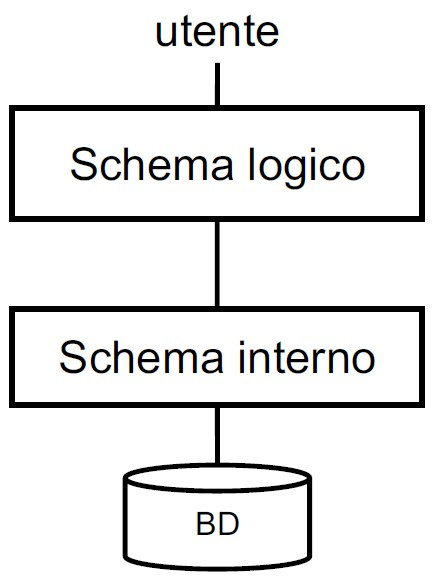
\includegraphics[width=0.5\textwidth]{img/MR_intro2.jpg}
\end{center}

\subsection{Indipendenza dei dati}
Il livello logico è \textbf{indipendente} da quello fisico:
\begin{itemize}
    \item una tabella è utilizzata nello stesso modo qualunque sia la sua realizzazione fisica (che può anche cambiare nel tempo)
    \item Perciò in questo corso vedremo solo il livello logico e non quello fisico
\end{itemize}

\subsection{I modelli logici dei dati}
Tre modelli logici tradizionali:
\begin{description}
    \item[gerarchico:] organizzazione ad albero
    \item[reticolare:] organizzazione a grafo
    \item[relazionale:] organizzazione a tabella
\end{description}
Più recenti (e meno diffusi):
\begin{description}
    \item[oggettuale:] organizzazione ad oggetti
    \item[XML] 
    \item[NoSQL:] basata su documenti
\end{description}
Si chiamano modelli \underline{logici} perché pur basandosi su strutture astratte queste riflettono una particolare organizzazione.
\\https://db-engines.com/en/ranking


\subsection{Il modello relazionale}
Permette di definire tipi per mezzo del costruttore \textbf{relazione} che permette di organizzare i dati in insiemi di record a \textit{struttura fissa}.
\\Una relazione è spesso rappresentata da una \textbf{tabella} (solo in questo specifico caso usabile come sinonimo di \textbf{relazione}):
\begin{itemize}
    \item le righe: rappresentano specifici record
    \item le colonne: corrispondono ai campi dei record
\end{itemize}
L'ordine di righe e colonne è sostanzialmente \textit{irrilevante}.
\begin{center}
    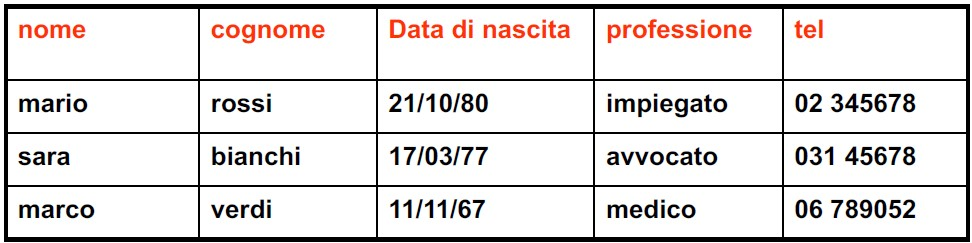
\includegraphics[width=0.5\textwidth]{img/MR_intro1.jpg}
\end{center}
In una base di dati relazionale ci sono in generale più relazioni.

\subsubsection{Un po' di storia}
Proposto da E. F. Codd nel 1970 per favorire \textit{l'indipendenza dei dati}.
\\Disponibile in DBMS reali nel 1981 (non è facile implementare l'indipendenza con efficienza e affidabilità!)
\\Basato:
\begin{itemize}
    \item sul concetto matematico di relazione - concetto formale (con una variante)
    \item tabelle - concetto intuitivo
\end{itemize}
Definisce come sono organizzati i dati e non come sono poi memorizzati e gestiti dal sistema informatico.

\subsection{Termine "relazione" in tre accezioni}
\begin{description}
    \item[relazione matematica:] come nella teoria degli insiemi
    \item[relazione:] secondo il modello relazionale dei dati
    \item[associazione o correlazione:] relazione (dall'inglese \textit{relationship}) che rappresenta una classe di fatti, nel modello Entity-Relationship.   
\end{description}

\chapter{Modello Relazionale - MR}
\subsection{Prodotto Cartesiano}
Dati due insiemi $D_1, D_2$ (Estendibile a $n$ insiemi distinti o non), definiamo nei seguenti modi:
\begin{itemize}
    \item Prodotto cartesiano $D_1 \times D_2$:
    \\L'insieme di tutte le coppie \textbf{ordinate} $(v_1, v_2)$ tali che $v_1 \in D_1$ e $v_2 \in D_2$
    \item Esempio $$A = {1,\, 2,\, 4}\, e\, B = {a,\, b}$$ Il prodotto cartesiano $A \times B$ è composto da: $${(1,a), (1,b), (2,a), (2,b), (3,a), (3,b)},$$ ovvero sei coppie ordinate (il primo da A, il secondo da B) senza ripetizioni.
\end{itemize}

\subsection{Relazione matematica}
\begin{itemize}
    \item $D1, …, Dn$ ($n$ insiemi anche non distinti)
    \item prodotto cartesiano $D_1 \times \cdot \times D_n$:
    \\l'insieme di tutte le $n$-uple ordinate $(d_1, \cdot, d_n)$ tali che $d_1 \in D_1, \cdot, d_n \in D_n$
    \item relazione matematica su $D_1, \cdot, D_n$:
    \\un sottoinsieme di $D_1 \times \cdot \times D_n$, ovvero del prodotto cartesiano.
    \item $D_1, \cdot, D_n$ sono i domini della relazione
Il numero delle componenti del prodotto ($n$) è detto \textbf{grado} della relazione; il numero di $n$-uple della relazione è la \textbf{cardinalità} della relazione.

\subsubsection{Es.:}

\subsubsection{Es. numeri di telefono:}

\subsubsection{Rel. matematica: alcune proprietà}
Una relazione matematica è un insieme di n-uple ordinate: (d1, …, dn) tali che d1ÎD1, …, dn Î Dn
\\Alcune proprietà:
\begin{itemize}
    \item non c'è ordinamento fra le n-uple (in verticale);
    \item le n-uple sono distinte;
    \item ciascuna n-upla è ordinata (in orizzontale): l'i-esimo valore proviene dall'i-esimo dominio.
\end{itemize}
L'ultima proprietà ci dice che ciascuno dei domini ha due ruoli diversi, distinguibili attraverso la posizione: ovvero, la struttura è \textbf{posizionale}. Scambiare la posizione fa variare il risultato, portando quindi a possibili errori.
\\Questo si può sistemare aggiungendo alla tabella una riga di \textbf{intestazione}:
\begin{itemize}
    \item a ciascun dominio si associa un nome (attributo), che ne descrive il "ruolo";
    \item gli attributi possono essere usati come intestazione;
    \item la struttura in questo modo non è più posizionale.
\end{itemize}

\subsection{Modello basato su valori}
Immagine
\subsubsection{Vantaggi:}
Indipendenza dalle strutture fisiche (si potrebbe avere anche 
con puntatori di alto livello) che possono cambiare
dinamicamente
• si rappresenta solo ciò che è rilevante dal punto di vista
dell'applicazione
• i dati sono portabili piu' facilmente da un sistema ad un altro
• per accedere ai dati non serve sapere come sono memorizzati
fisicamente
\subsection{Modello basato su puntatori}
Immagine

\subsection{Schema e istanza}
In ogni base di dati esistono:
• lo schema, sostanzialmente invariante nel tempo, che ne
descrive la struttura (aspetto intensionale). Scritto con la lettera maiuscola.
• es.: le intestazioni delle tabelle
• l'istanza, i valori attuali, che possono cambiare anche
molto rapidamente (aspetto estensionale). Scritto con la lettera minuscola.
• es.: il “corpo” di ciascuna tabella

\subsubsection{Definizioni}
Schema di relazione:
un nome R1 (MAIUSCOLO) con un insieme di attributi
X={A1, ..., An}:
R1(A1,..., An) = R1(X)
% immagine
Schema di base di dati:
insieme di schemi di relazione con nomi diversi:
R = {R1(X1), ..., Rk(Xk)}
% immagine
Una tupla su un insieme di attributi X è una funzione t che associa a
ciascun attributo A in X un valore del dominio di A
• t[A] (o t.A) denota il valore della tupla t sull'attributo A
% immagine
una relazione R con attributi A1, A2 e A3, e corrispondenti
domini D1, D2 e D3 si può denotare anche come
R(A1 : D1, A2 : D2, A3 : D3)

(Istanza di) relazione su uno schema R(X):
insieme r1 (minuscolo) di tuple su X
• (Istanza di) base di dati su uno schema R= {R1(X1), ..., Rn(Xn)}:
insieme di relazioni r = {r1,..., rn} (con ri relazione su Ri)

\subsection{Un po' di notazione}


\subsection{Tabelle e relazioni}
Una tabella rappresenta una relazione se
\begin{itemize}
    \item i valori di ogni colonna sono fra loro omogenei
    \item le righe sono diverse fra loro
    \item le intestazioni delle colonne sono diverse tra loro
\end{itemize}
In una tabella che rappresenta una relazione
\begin{itemize}
    \item l'ordinamento tra le righe è irrilevante
    \item l'ordinamento tra le colonne è irrilevante
\end{itemize}

\subsubsection{Chiave}
insieme di attributi che identificano univocamente le tuple di
una relazione
Formalmente:
• un insieme K di attributi è superchiave per r se r non
contiene due tuple distinte t1 e t2 con t1[K] = t2[K]
• K é chiave per r se è una superchiave minimale per r (cioé non contiene un'altra superchiave)
% tre esempi
Ma data una tabella qualsiasi, esiste sempre una superchiave (\textbf{NON} minimale)? Dato che la tabella proviene da un prodotto cartesiano e nel prodotto cartesiano non ci sono ripetizioni, allora possiamo dire che la risposta è sì. E la superchiave corrisponderà all'insieme di \textbf{tutti} gli attributi della tanella.
\\All'esame ci verranno dati schemi di relazione, dobbiamo individuarne la superchiave e i vincoli.

\subsubsection{Informazione incompleta}
ll modello relazionale impone ai dati una struttura rigida:
\begin{itemize}
    \item le informazioni sono rappresentate per mezzo di tuple
    \item solo alcuni formati di tuple sono ammessi: quelli che corrispondono agli schemi di relazione
\end{itemize}
I dati disponibili possono non corrispondere al formato previsto:
\begin{itemize}
    \item Hanno attributi in più che non sono nello schema
    \item Mancano di alcuni attributi = Informazione incompleta
\end{itemize}

\subsubsection{Informazione incompleta: motivazioni}
% immagine

\subsubsection{Informazione incompleta nel modello relazionale}
Si adotta una tecnica rudimentale ma efficace:
• valore nullo: denota l'assenza di un valore del dominio
(e non è un valore del dominio)
• t[A], per ogni attributo A, è un valore del dominio dom(A)
oppure il valore nullo NULL

e altre cose

tutti questi vincoli ci aiutano a gestire la bd in modo che i dati non siano incosistenti.

tipi di vincoli:

per la slide 61, all'esame va bene così com'è nella slide oppure in linguaggio naturale
